\section{Test cases for complex statecharts: hierarchy}
\label{testHierarchy}

In this section, the generation of test cases for statecharts that comprise the hierarchy feature is described (a state may contain many substates and so on). We do not limit the level of nested hierarchy for the automatic generation. Consider states $a$ and $b$, such that $a$ contains $b$. We will say that $a$ is the superstate of $b$ and $b$ is the substate of $a$.

One way to deal with hierarchy is eliminating it from the model by flattening the statechart, as shown in \ref{flattening}. If so, the statechart becomes an automaton and the techniques for simple statecharts explained in the previous section can be used. Instead, the approach taken in the present project is keeping the structure of the statechart and creating the test cases incrementally, following the technique described in \cite{bogdanov}.

Similarly to the previous case, we need to cover all states by constructing the set $C$ and then test all transitions in the model. The construction of $C$, however, needs to take into account states and all their corresponding substates in order to provide the whole coverage. It is important to note that we considered only statecharts that do not have transitions between different hierarchy levels. 

Given a state, we first check if it contains substates. If it does, we can compute substates' coverage paths going deeper in the hierarchy level. Later, we concatenate the coverage path of the superstate to each coverage path of the substates. Then, the coverage path of the superstate should be removed from $C$ and the paths of the substates will be kept in $C$ instead. If the coverage path $p$ of a certain state $s$ passes through a superstate $q$, we need to mark in $p$ that it passed by $q$ and that the coverage paths of $q$'s substates should be used when creating test cases for transitions leaving $s$. To mark that, we will use the notation $\Delta_q$

The algorithm to construct $C$ is changed accordingly to comprise these new features: 

\begin{lstlisting}[mathescape,caption={Recursive State Cover construction for statecharts with hierarchy}]
//Recursive function that will do all the work
//returns the State Cover set, or set C
Set constructSetCRec(State s, Path p, Set setC, List visited) {

	visited.add(s);

	setC.add(s,p);

	if (s.containsSubstates()) {

		Set subSetC = constructSetC(s.getInitialSubstate());	

		s.addSubpaths(subSetC);

		setC.remove(s,p);

		for (State substate in s.getSubstates()) {

			Path partialPath = subSetC.getPath(substate);

			Path substateCoveragePath = p + partialPath;

			setC.add(substate,substateCoveragePath)	
		}
		
	}
	
	for (Transition t in s.getOutgGoingTransitions()) {
		
		State nextState = t.getDestiny();

		if (!visited.contains(nextState)) {

			if (s.containsSubstates()) {
			
				Path nextCoveragePath = p + $\Delta_{s}$ + t.getLabel());

			} else {

				Path nextCoveragePath = p + t.getLabel());

			}	

			constructSetCRec(nextState,nextCoveragePath,setC,visited);	
		}
	}
	
	return setC;
}

\end{lstlisting}
 

Once the set $C$ is complete, we can create the test cases based on every transition that leaves each state. In states with no substates and whose coverage did not pass by any superstate, the previous process (presented in \ref{pseudocodeTestCase}) is applied.

On the other hand, if the state's coverage path $p$ went through a superstate $s$, we need to expand the path with the coverage paths of the substates. In other words, for each substate with coverage path $u$,  there will be a $p'$ with $u$ replacing the notation $\Delta_s$, where $s$ is the superstate. The algorithm for the expansion is:

\begin{lstlisting}[mathescape,caption={Expansion psseudocode for a path that passes through a superstate}]
//Pseudocode for an expansion function
//Receives the original, not expanded, path and the super state it passes through
//Returns the set of paths resulting from the expansion
Set pathExpansion(Path originalPath, State superState) {
		
	Set subPaths = superState.getSubpaths();

	Set expansionResults = new Set();

	for (State substate in superState.getSubstates()) {
		
		Path subPath = subPaths.getPath(substate);

		Path expanded = originalPath.replace($\Delta_{superState}$, subPath);

		expansionResults.add(expanded);
	}

	return expansionResults;
}

\end{lstlisting}

If a state contains substates, however, we must transfer the origin of every transition that leaves it to each one of its substates. Consider the case that a state $s$ has a transition $t = (s,l,q)$ and contains substates $s_1, s_2$ and $s_3$. When creating the test case for $t$, we must actually consider three new transitions: $t_1 = (s_1,l,q), t_2 = (s_2,l,q)$ and $t_3 = (s_3,l,q)$. The pseudocode to transfer transitions from the superstate to the substates is presented below:

\begin{lstlisting}[caption={Pseudocode to transfer transitions from a superstate to its substates}]
//Add all transitions of a superstate in its substates
//Receives the superstate as argument
void transferFromSuperToSub(State super) {
	
	for (Transition t in super.getOutgGoingTransitions()) {
		
		for (State sub in super.getSubstates()) {
			
			sub.addOutGoingTransition(t);
		}
	}
}

\end{lstlisting}

The pseudocode to create the final test cases is the same as the one presented in \ref{pseudocodeTestCase}.

Let's take the statechart in Figure \ref{fig:webEDI} to illustrate the technique. It models an application that receives order files in an specific format and converts them into a well formatted xml. Each order file contains several lines, and each line contains a product and its corresponding amount. The application also has an integration layer: it receives the xml file and then send it to the management system. This statechart models the requirement described in Subsection \ref{req3}.

\begin{figure}[htb]
\centering
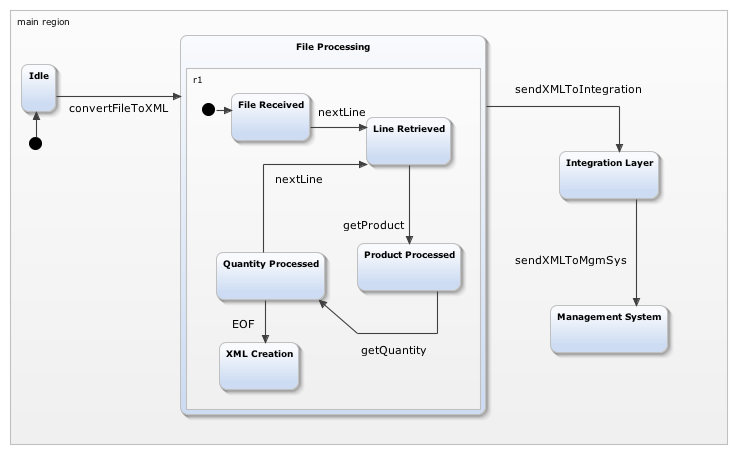
\includegraphics[width=15cm]{figuras/webEDI}
\caption{\label{fig:webEDI} Statechart for order file processing and transference}
\end{figure}

Now, to construct the coverage path to \textit{Idle} we do not need to worry about hierarchy, so approach described in the prior Section \ref{testSimpeState} is enough.

\begin{center}
\begin{tabular}{| l | l|}

\hline

State & Coverage path \\ \hline

Idle & e \\

\hline
\end{tabular}
\end{center}

Notice that once again the empty string $e$ is present due to the default unlabelled transition entering the \textit{Idle} state.
%
When creating the coverage path for state \textit{File processing}, however, we realise that it is a superstate. So, we go deeper in the hierarchy level to obtain the coverage paths of substates \textit{File received, Line retrieved, Product processed, Quantity processed} and \textit{XML creation}. Then,  the following paths are added to set $C$:

\begin{center}
\begin{tabular}{| l | l|}

\hline

State & Coverage path \\ \hline

File received & e convertFileToXML e \\ \hline

Line retrieved & e convertFileToXML e nextLine\\ \hline

Product processed & e convertFileToXML e nextLine getProduct\\ \hline

Quantity processed & e convertFileToXML e nextLine getProduct getQuantity\\ \hline

XML creation & e convertFileToXML e nextLine getProduct getQuantity EOF\\ 

\hline
\end{tabular}
\end{center}

Note that the coverage path for the superstate \textit{File processing} is removed from $C$ because we are considering its substates. Therefore, the test cases that would be created based on the superstate will be created based on the substates, instead. Also, the empty string $e$ is added twice in each of these paths. This is necessary because these paths pass through two default unlabelled transitions: the first one entering the \textit{Idle} state, and the second one entering \textit{File processing}.

Now, states \textit{Integration layer} and \textit{Management system} must also be covered. Observe that to cover these states, we need to pass by \textit{File processing}, a superstate. Therefore, in their coverage path, we need to use an specific notation to guide the later expansion with the substates coverage paths. Notation $\Delta_{File\ processing}$ is used for this particular purpose. When creating the test cases, we need to expand the path considering the coverage of \textit{File processing}'s substates. Thus, the coverage paths for the \textit{Integration layer} and \textit{Management system} states are:

\begin{center}
\begin{tabular}{| l | p{10cm}|}

\hline

State & Coverage path \\ \hline

Integration layer & e convertFileToXML $\Delta_{File\ processing}$ sendXMLToIntegration \\ \hline

Management system & e convertFileToXML $\Delta_{File\ processing}$ sendXMLToIntegration sendXMLToMgmSys\\

\hline
\end{tabular}
\end{center}

At this point, when the set $C$ is complete, we can actually create the test cases. To illustrate this, we will examine transitions \textit{getProduct, sendXMLToIntegration} and \textit{sendXMLToMgmSys} more closely.

For \textit{getProduct}, a transition leaving a substate, the process will be the same as the one presented in the pseudocode \ref{pseudocodeTestCase}. Hence, we have the following test case:

\begin{itemize}

\item Test case for \textit{\textbf{getProduct}}

Origin state: \textit{Line Retrieved}

Test Path: \textit{e convertFileToXML e nextLine getProduct}

Expected state: \textit{Product processed}

\end{itemize}

In the case of \textit{sendXMLToIntegration}, a transition that leaves a superstate, we need to use the information regarding the substates to create the test cases. For each substate's coverage path $p$, there will be a test case for \textit{sendXMLToIntegration} using $p$. Then, $sendXMLToIntegration$ is appended to each $p$ in order to obtain the test paths:

\begin{itemize}

\item Test case \#1 for \textit{\textbf{sendXMLToIntegration}}

Origin state: \textit{File Received}

Test Path: \textit{e convertFileToXML e sendXMLToIntegration}

Expected state: \textit{Integration layer}

\item Test case \#2 for \textit{\textbf{sendXMLToIntegration}}

Origin state: \textit{Line Retrieved}

Test Path: \textit{e convertFileToXML e  nextLine sendXMLToIntegration}

Expected state: \textit{Integration layer}


\item Test case \#3 for \textit{\textbf{sendXMLToIntegration}}

Origin state: \textit{Product Processed}

Test Path: \textit{e convertFileToXML e  nextLine  getProduct sendXMLToIntegration}

Expected state: \textit{Integration layer}

\item Test case \#4 for \textit{\textbf{sendXMLToIntegration}}

Origin state: \textit{Quantity Processed}

Test Path: \textit{e convertFileToXML e  nextLine  getProduct  getQuantity sendXMLToIntegration}

Expected state: \textit{Integration layer}

\item Test case \#5 for \textit{\textbf{sendXMLToIntegration}}

Origin state: \textit{XML Creation}

Test Path: \textit{e convertFileToXML e  nextLine  getProduct  getQuantity EOF sendXMLToIntegration}

Expected state: \textit{Integration layer}

\end{itemize}

As for transition \textit{sendXMLToMgmSys}, the expansion of \textit{Integration layer}'s coverage path is pending. Similarly to what we did for the transition \textit{sendXMLToIntegration}, we also need to consider the paths of \textit{File processing}'s substates. Therefore, the test cases for \textit{sendXMLToMgmSys} are:

\begin{itemize}

\item Test case \#1 for \textit{\textbf{sendXMLToMgmSys}}

Origin state: \textit{Integration Layer}

Test Path: \textit{e convertFileToXML e sendXMLToIntegration sendXMLToMgmSys}

Expected state: \textit{Integration layer}

\item Test case \#2 for \textit{\textbf{sendXMLToMgmSys}}

Origin state: \textit{Integration Layer}

Test Path: \textit{e convertFileToXML e  nextLine sendXMLToIntegration sendXMLToMgmSys sendXMLToMgmSys}

Expected state: \textit{Integration layer}


\item Test case \#3 for \textit{\textbf{sendXMLToMgmSys}}

Origin state: \textit{Integration Layer}

Test Path: \textit{e convertFileToXML e  nextLine  getProduct sendXMLToIntegration sendXMLToMgmSys}

Expected state: \textit{Integration layer}

\item Test case \#4 for \textit{\textbf{sendXMLToMgmSys}}

Origin state: \textit{Integration Layer}

Test Path: \textit{e convertFileToXML e  nextLine  getProduct  getQuantity sendXMLToIntegration sendXMLToMgmSys}

Expected state: \textit{Integration layer}

\item Test case \#5 for \textit{\textbf{sendXMLToMgmSys}}

Origin state: \textit{Integration Layer}

Test Path: \textit{e convertFileToXML e  nextLine  getProduct  getQuantity EOF sendXMLToIntegration sendXMLToMgmSys}

Expected state: \textit{Integration layer}

\end{itemize}

Notice that, in each case, $\Delta_{File\ processing}$ in the \textit{Integration layer}'s coverage was replaced by a substate's coverage path.

